\chapter{Durchführung}
\label{cha:Durchführung}
\section{Versuchsaufbau}
\label{sec:aufbau}
Der Versuchsaufbau zur Bestimmung der Kernspins von Rubidium-Isotopen ist in Abbildung \ref{fig:aufbau_v21} dargestellt.

\begin{figure}
              \centering
              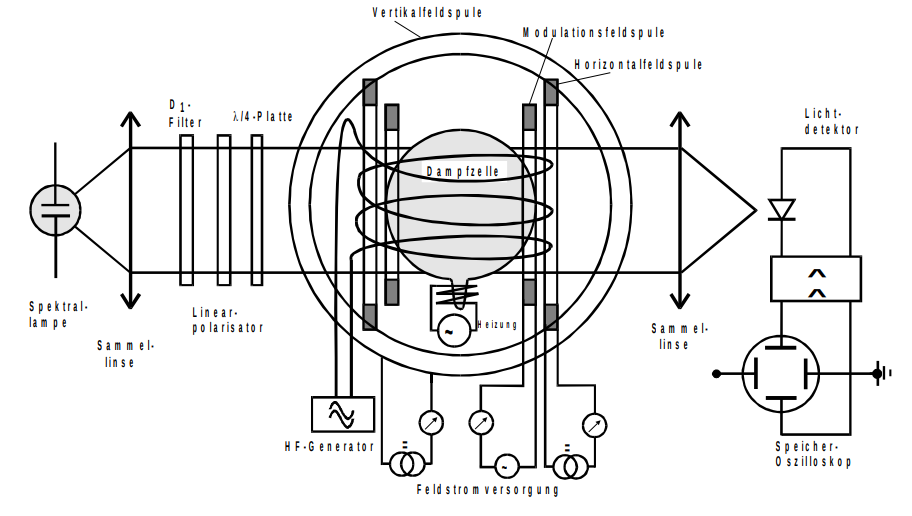
\includegraphics[width = \textwidth]{content/v21_bilder/aufbau.PNG}
              \caption{Skizze des Aufbaus zur Messung der Kernspins von Rubidium. \cite{v21}}
              \label{fig:aufbau_v21}
\end{figure}

Zunächst muss das Licht für optisches Pumpen erzeugt werden. Dazu wird $D_1$-Licht benötigt, weches bei dem Übergang vom $p$ ins $s$ Niveau bei Rubidium entsteht. Daher wird eine 
Rubidium-Spektral-Lampe verwendet. Da diese divergentes Licht austrahlt wird danach eine Sammellinse verwendet um kolineare Licht zu erhalten. Danach trifft das Licht auf einen 
$D_1$-Filter, welcher nochmal dafür sorgt, dass wirklich nur $D_1$-Licht propagiert um Fehler zu minimieren. Da der $\sigma^+$ übergang nur durch rechtszirkular-polarisiertes Licht 
angeregt werden kann muss das Licht noch polarisiert werden. Dazu wird eine Kombination aus einem Linearpolarisator und einer $\frac{\lambda}{4}$-Platte. Das resultierende Licht kann 
dann auf die Dampfzelle, in welcher sich ein Gasgemisch aus den Rubidium-Isotopen befindet. Um diese Zelle befindet sich zunächst eine Spule, welche ein vertikales Magnetfeld 
erzeugt. Dieses Feld soll das Erdmagnetfeld kompensieren. Außerdem werden zwei weitere Spulen verwendet, welche ein Magnetfeld in horizontaler Richtung erzeugen. Dabei handelt es sich 
bei einer Spule um eine einfache Helmholtzspule, welche ein konstantes Magnetfeld liefern soll. Die andere Spule ist ebenfalls eine Helmholtzspule, aber diese ist so konstruiert, dass
ihr Magnetfeld sehr einfach variiert werden kann. Diese Spule wird Sweep-Spule genannt. Das gesamte horizontale Feld wird RF-Feld genannt.

Nachdem das Licht die Dampfzelle durchdringt, oder auch nicht durchdringt, trifft es auf eine weitere Linse um das Licht auf ein
Si-Photoelement zu fokussieren, welches die Intensität in eine Spannung konvertiert. Diese Spannung kann dann am Oszilloskop sichtbar gemacht werden. 

\section{Messanleitung}
\label{sec:messanleitung}
Zunächst muss das Erdmagnetfeld in horizontale Richtung kompensiert werden. Dauz wird der Versuchsaufbau lediglich gedreht, sodass dieser nach Norden ausgerichtet ist. Dadurch verschwindet
die horizontale Komponente. Nun wird das vertikale Magnetfeld durch die dafür vorgesehene Spule kompensiert. Dabei muss darauf geachtet werden, dass der Peak am Oszilloskop möglichst 
schmal wird. Nun können die horizontalen Spulen eingeschaltet werden und die Messung begonnen werden. Dabei muss bei Frequenzen von $\qty{100}{\kilo\hertz}$ bis zu $\qty{1}{\giga\hertz}$ 
jeweils das resonante Magnetfeld durch die Sweepspule eingestellt werden. Dieses kann am Oszilloskop eingestellt werden, indem der Messpunkt direkt in die Peaks gefahren wird und dann das 
Magnetfeld abgelesen wird. Diese Messung wird in $\qty{100}{\kilo\hertz}$ Abständen wiederholt. Zuletzt wird noch einmal eine Frequenz von $\qty{100}{\kilo\hertz}$ eingestellt und das Bild 
am Oszilloskop gespeichert. Anhand des Amplitude der Peaks kann das Isotopenverhältnis bestimmt werden. 